\section{First application: changing the source}
\label{main:construction}

The first application follows the design procedure of Section~\ref{main:chain} step by step. A disconnected source forces transitions (Section~\ref{main:source}); choosing the unit cube, a connected volume, removes that structural cause. The composition rules then state what the remaining links must supply. The tool path $x=\Phi\circ\xi$ is continuous only if both the traversal and the geometry map are, and by \eqref{eq:main-measure} it has the prescribed occupation measure only if
\begin{equation}
  \label{eq:main-volume-obligations}
  \xi_\#\lambda^1=\lambda^3,\qquad \Phi_\#\lambda^3=\mu_\Omega ,
\end{equation}
where $\lambda^3$ is uniform volume on the cube. The traversal must therefore be a continuous, measure-preserving curve through the cube, and the geometry map must be a continuous map that pushes uniform volume onto $\mu_\Omega$. A space-filling curve meets the first obligation exactly, and optimal transport meets the second, with continuity under the convexity assumptions below. The resulting \emph{transported Hilbert path}, or transported path for short, gives each map a single job: the traversal orders, and the geometry map shapes. The construction ends at the tool path: the lift and the process remain abstract links of the chain.

\subsection{Construction: Hilbert orders, transport shapes}
The traversal is the three-dimensional Hilbert curve $\Hil$ \cite{hilbert1891,sagan1994,bader2013}. It visits every point of the cube continuously, spends equal time in equal volumes, and keeps points visited at nearby times close together. At a finite order $m$ it visits the centres $u_1,\dots,u_n$ of $n=8^m$ cells, consecutive cells sharing a face \cite{haverkort2017}; Appendix~\ref{sec:vsfc-hilbert} establishes its measure preservation, locality, and finite-order estimates. Here the geometry map $\Phi$ is chosen as the optimal-transport map. Among all maps that send uniform volume in the cube to the target distribution $\mu_\Omega$, it minimises the mean squared displacement \cite{brenier1991,peyre2019computational}. The transported path is
\begin{equation}
  \label{eq:main-vsfc}
  x(t)=\Phi\bigl(\Hil(t)\bigr).
\end{equation}

\begin{figure}[tb]
  \centering
  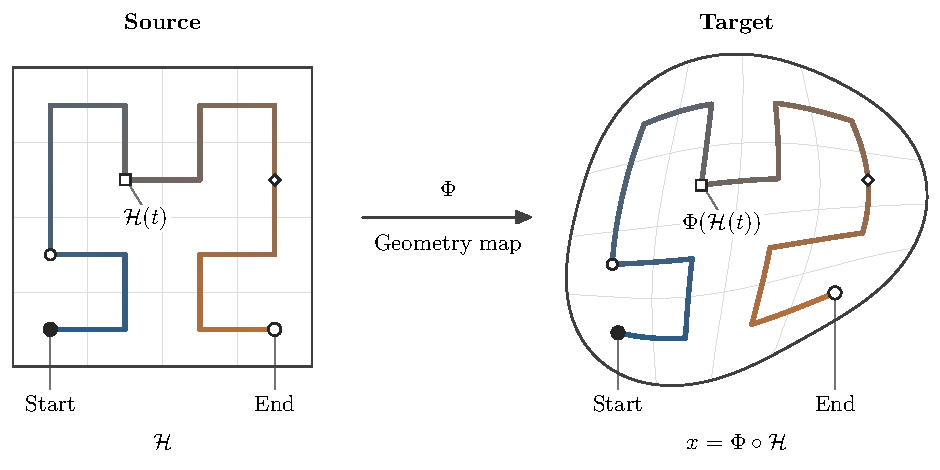
\includegraphics[width=\textwidth]{figures/hilbert_transport.pdf}
  \caption{Hilbert orders, transport shapes. A numerical two-dimensional illustration of the volumetric construction: an order-two Hilbert traversal $\mathcal H$ in the source square (left) is carried into the target by a smooth approximation of the geometry map $\Phi$ (right), computed from an entropically regularised quadratic optimal-transport solve. Matching colours and marker shapes indicate corresponding traversal times; the visiting order is inherited from the source.}
  \label{fig:hilbert-transport}
\end{figure}

Composition gives $x_\#\lambda^1=\Phi{}_\#\lambda^3=\mu_\Omega$; when transport is continuous, the composed path is continuous as well. Figure~\ref{fig:hilbert-transport} illustrates the construction numerically in two dimensions, and Figure~\ref{fig:teaser} (top) illustrates the construction on the Stanford bunny. Its distinction is to transport a traversed volume while preserving the prescribed occupation measure: earlier manufacturing uses of Hilbert curves traverse layers or deposition surfaces \cite{bertoldi1998domain,papacharalampopoulos2018path}, while curved-layer, multi-axis, and neural slicers deform layers \cite{etienne2019curvi,zhang2022s3,liu2024neural}.

\subsection{Guarantees on convex parts}
\label{main:convex}
The Hilbert curve is continuous, so the transported path is continuous wherever the transport map is. Optimal transport always delivers the prescribed distribution, but it need not be continuous: a map that sends a cube onto a shape with a hole may have to tear. Convex targets avoid this. If the part is compact and convex with nonempty interior, and the target density is bounded above and below by positive constants, the transport map is H\"older continuous on the closed cube \cite{caffarelli1992,jhaveri2022regularity}; Appendix~\ref{app:proofs-convex-transport} explains why these assumptions suffice. We call these assumptions the \emph{convex setting}.

In the convex setting, the ideal transported path is continuous and has the prescribed occupation measure, $x_\#\lambda^1=\mu_\Omega$; Appendix~\ref{sec:vsfc-certificates} derives this (Theorem~\ref{thm:vsfc-guarantees}(ii)) together with the finite-order bounds below. Physically, the nozzle never has to break off and travel: the path has no stop, and the time it spends in each region matches the prescription.

At a finite Hilbert order $m$, the guarantee becomes a bound. Waypoints $\hat x_i$ that lie within $\varepsilon$ of $\Phi(u_i)$ satisfy, for constants $\beta\in(0,1]$ and $C_\Phi$ (Theorem~\ref{thm:vsfc-guarantees}(i)),
\begin{equation}
  \label{eq:main-bounds}
  \text{covering radius}\leq C_\Phi2^{-\beta m}+\varepsilon,\qquad
  \text{step length}\leq C_\Phi2^{-\beta m}+2\varepsilon .
\end{equation}
The two terms belong to different links. A finer Hilbert order shrinks the first; only a more accurate geometry map shrinks the second. The constants are not known for a computed map, which is why the computation below supplies a bound of its own.

Outside the convex setting, the guarantee is absent rather than refuted: transport still delivers the prescribed distribution, but no theorem makes it continuous. Implementing the construction also requires computing the map, which brings its own certificates and its own gaps.

\subsection{Implementation: semi-discrete transport}
\label{main:semidiscrete}
The waypoints are computed by semi-discrete optimal transport between the part and the finite Hilbert curve \cite{aurenhammer1998minkowski,merigot2011multiscale,levy2015numerical}. The order-$m$ curve is the discrete measure $\nu_m=n^{-1}\sum_i\delta_{u_i}$, one unit of time per site, and the part carries the continuous target $\mu_\Omega=\rho\,dy$, which may be graded. For weights $\psi\in\mathbb R^n$, the \emph{Laguerre cell} of site $u_i$ is the part of $\Omega$ that is power-nearest to it,
\begin{equation}
  \label{eq:main-laguerre}
  L_i(\psi)=\bigl\{y\in\Omega:\ \|y-u_i\|^2-\psi_i\leq\|y-u_j\|^2-\psi_j\ \text{for all }j\bigr\}.
\end{equation}
The cells always tile $\Omega$. The solver adjusts $\psi$ until every cell carries its site's share of the target, up to solver tolerance,
\begin{equation}
  \label{eq:main-equal-mass}
  \mu_\Omega\bigl(L_i(\psi)\bigr)=\tfrac1n\qquad(i=1,\dots,n),
\end{equation}
which makes the map sending each $L_i$ to $u_i$ the optimal transport from $\mu_\Omega$ to $\nu_m$ \cite{aurenhammer1998minkowski,peyre2019computational}. Each Hilbert site is finally replaced by the density-weighted centroid of its cell,
\begin{equation}
  \label{eq:main-centroid}
  \hat x_i=n\int_{L_i(\psi)}y\,\rho(y)\,dy ,
\end{equation}
and the waypoints are visited in Hilbert order. A Hilbert site thus labels a cell of the part rather than serving as a waypoint, and the waypoint is the centre of mass of that cell. On the cube with uniform density, each cell is the Hilbert cell and $\hat x_i=u_i$: the construction is the identity, as it should be.

This construction controls, cell by cell, what the ideal map is meant to control; Appendix~\ref{sec:vsfc-semidiscrete} proves its distribution, order, and containment properties (Proposition~\ref{prop:sd-mass}) and the hull-gap bounds used below.
\begin{itemize}
  \item \emph{Cell mass.} Every waypoint stands for the same mass $1/n$ of the target, matching the equal time that the Hilbert curve spends in each cell. No target sample is drawn and none is deleted.
  \item \emph{A computable distribution bound.} Sending each cell's mass to its own centroid moves no mass farther than the largest cell diameter $D_m=\max_i\operatorname{diam}L_i(\psi)$, so the waypoints match the target to within $W_\infty\leq D_m$. Unlike $\varepsilon$ in \eqref{eq:main-bounds}, $D_m$ is measured for every computed path.
  \item \emph{Order.} Each centroid stays power-nearest to its own site, so the waypoints inherit the Hilbert labels without reordering.
\end{itemize}

Three things are not controlled, and the third becomes the turning point of the construction. First, how fast $\hat x_i$ approaches $\Phi(u_i)$ is not certified, so the step bound in \eqref{eq:main-bounds} remains conditional. Second, equal cell mass is not waypoint-density accuracy: regions thinner than a cell are not resolved (Proposition~\ref{prop:sd-mass}(iii)). Third, equal mass says nothing about containment. On a convex part each clipped cell is convex, so every centroid and every segment between consecutive centroids lies in the part. On a non-convex part, two mechanisms break this: a cell straddling a reentrant corner is clipped into disconnected portions whose combined centroid can lie in the empty region between them, and two cells with centroids inside the part can be joined by a segment that crosses a hole. Figure~\ref{fig:containment-repair} (Section~\ref{main:evidence}) shows both on computed paths.

\subsection{Repair: a volumetric source in several pieces}
\label{main:decomposed}
The chain assigns this failure to the geometry map, not the source: the cube is still connected, and the excursions arise where cells are clipped by holes and reentrant edges. The repair therefore stays within the first application: it restores the geometry map's convexity assumption, or nearly so, while keeping the source volumetric. Instead of one cube, the source becomes $k$ cubes, each transported onto a convex or near-convex piece of the part. Every piece is still filled by a path that runs through its volume; what changes is that the part now receives several piece paths instead of one. How far each piece may be from convex is measured by a single quantity.

\paragraph{A geometric guarantee for near-convex domains.}
For a compact domain $K$, let $\delta_K=\sup_{z\in\operatorname{conv}(K)}\dist(z,K)$ be its \emph{convex-hull gap}: how far its convex hull reaches beyond it. Centroids of cells contained in $K$, and straight segments joining them, lie in its convex hull, hence within distance $\delta_K$ of $K$ (Proposition~\ref{prop:sd-hull-gap}). This bound needs no transport regularity and recovers exact containment when $K$ is convex. It bounds excursion depth only.

\paragraph{The decomposed source.}
Given a partition of the part into $k$ convex or near-convex pieces $\Omega_1,\dots,\Omega_k$, the source is $k$ cubes, one per piece, and the Hilbert traversal and semi-discrete transport are applied independently to each (Figure~\ref{fig:teaser}, bottom). Each piece receives its share $w_j=\mu_\Omega(\Omega_j)$ of deposition time, and its path leaves it by at most its own hull gap $\delta_j$, with exact containment for convex pieces (Corollary~\ref{cor:sd-piece-hull-gap}).

Two kinds of excursion must now be kept apart. A piece path can leave its \emph{assigned piece}, by at most $\delta_j$; such an excursion may enter a neighbouring piece and so remain inside the part. Or it can leave the \emph{whole object}, which is the failure that decomposition is meant to remove. The hull-gap bound controls the first directly; it controls the second only where the region within $\delta_j$ of a piece lies inside the part.

\paragraph{The remaining tradeoff.}
Decomposition reintroduces separate pieces into the source, so Proposition~\ref{prop:topology-transitions} forces at least $k-1$ transitions between piece paths. Unlike the $N$ layers of a layered slicer, $k$ is set by the partition of the part, not by the Hilbert order, so the count does not grow as the resolution is refined. Sequencing the pieces, and hence executing these transitions, is outside the scope of this paper.
